\begin{figure}[!h]
    \vspace{-35pt}
    \hspace*{5mm}
    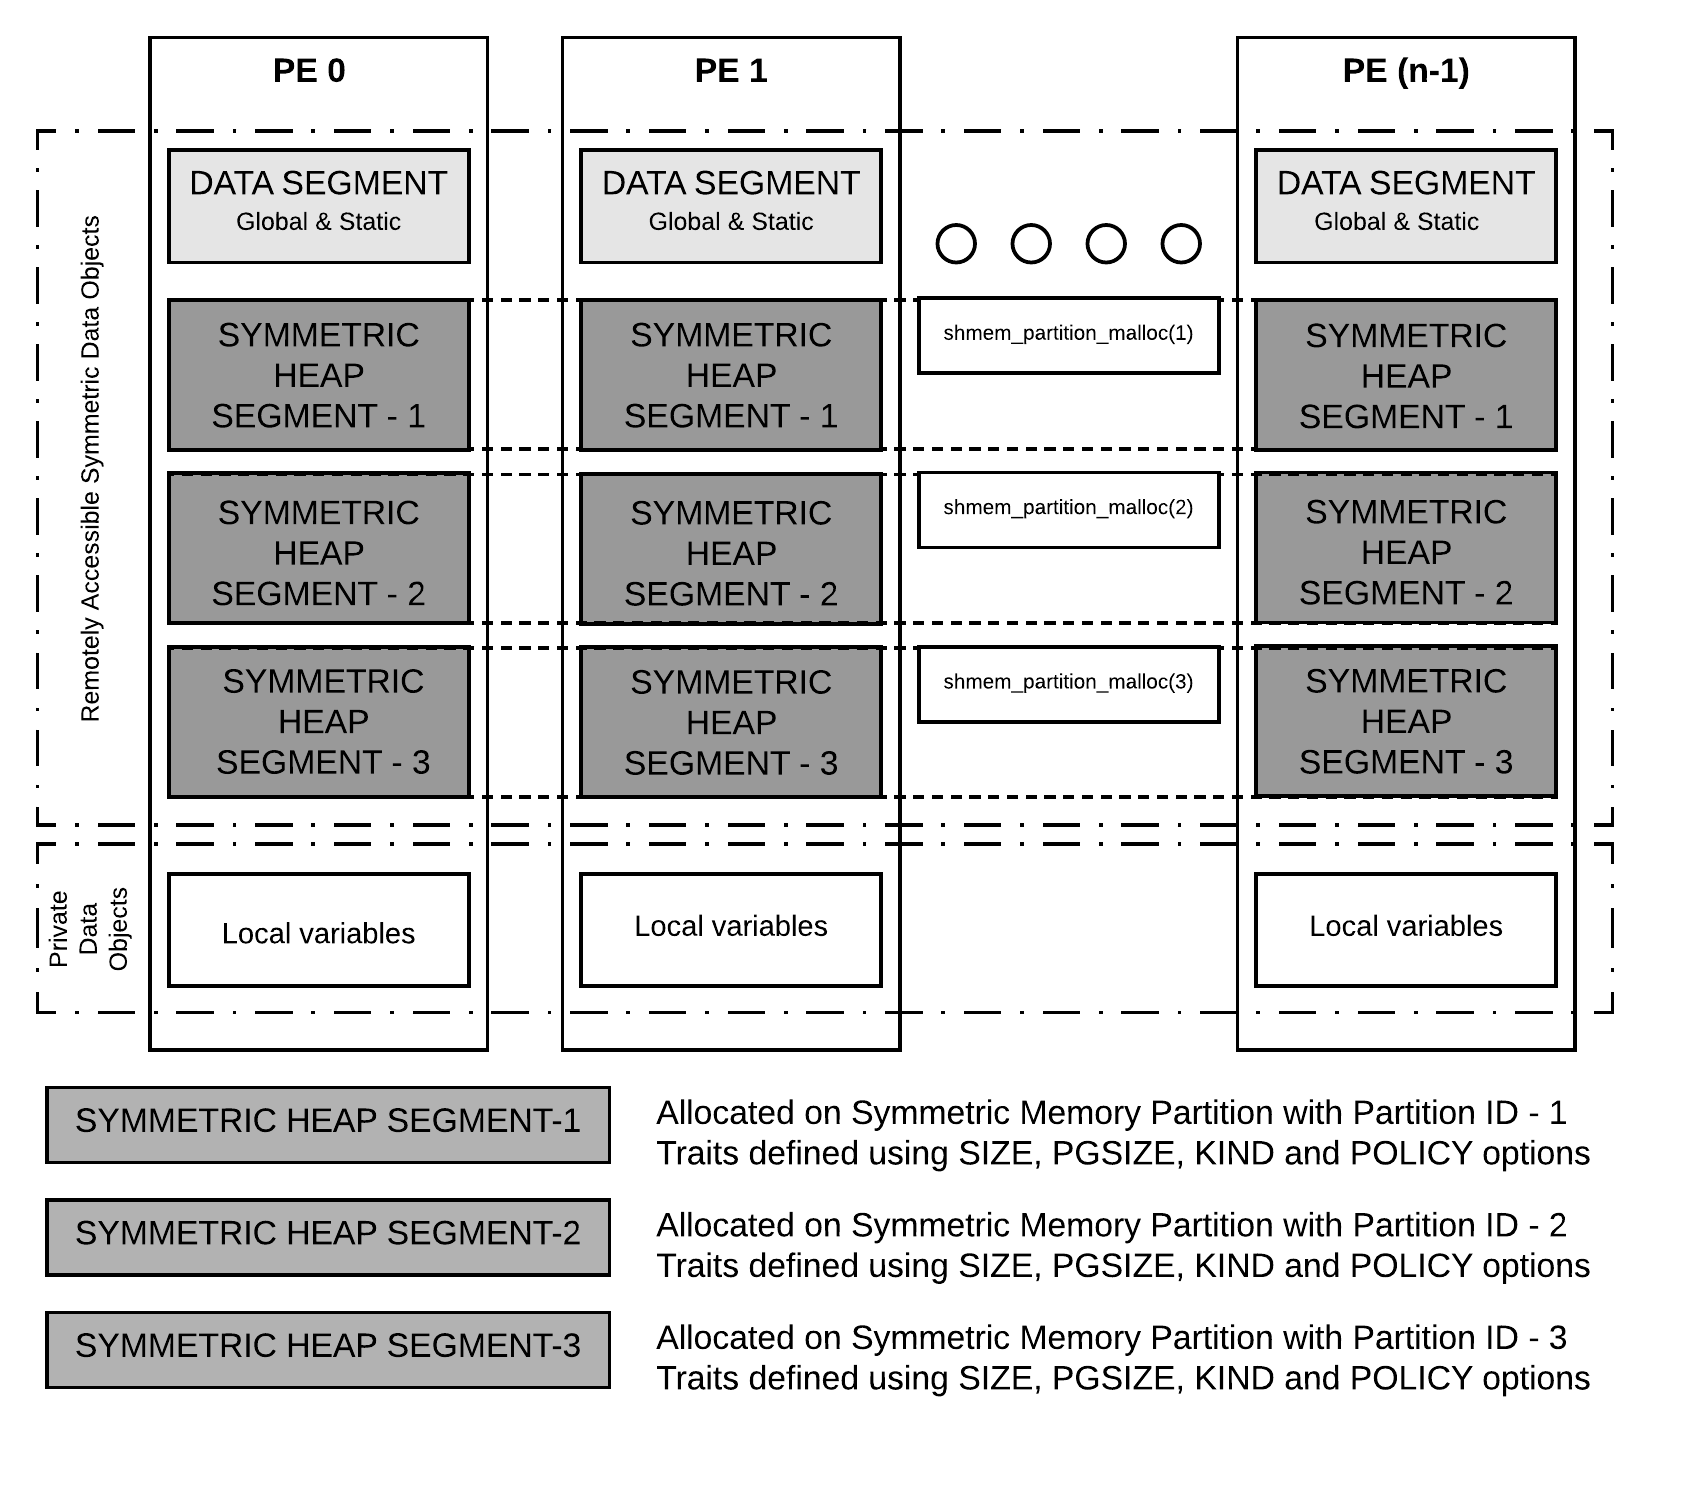
\includegraphics[scale=0.20]{image/smem-model.png}
    \vspace{-35pt}
    \caption{OpenSHMEM Memory Model with Symmetric Memory Partitions}
    \vspace{-25pt}
    \label{fig:smem-model}
\end{figure}

\section{Symmetric Memory Partitions in OpenSHMEM}
\label{src:smempart}

As mentioned in Section~\ref{src:mmodel}, the OpenSHMEM memory
model allows creation of one symmetric heap per PE during program
execution on a memory region determined by the implementation. The
only trait the user controls on the symmetric heap is the size.
This paper proposes a new feature called Symmetric Memory Partitions
to define the runtime changes and routines to support different
kinds of memory for the symmetric heap. Fig.~\ref{fig:smem-model}
shows the modified OpenSHMEM memory model and the proposed changes
are as follows:

\begin{itemize}
    \item symmetric heap is created on a single memory region
    determined by the implementation or on multiple memory regions
    determined by the users. The user-determined memory regions are
    called Symmetric Memory Partitions;
    \item only a single symmetric heap is created at each partition;
    \item multiple symmetric heaps are created by defining
    multiple separate symmetric memory partitions;
    \item each symmetric memory partition is identified using its
    \emph{Partition ID} label;
    \item each symmetric memory partition have their own memory
    traits to define the characteristics of each partition;
    \item apart from name, data type, and size attributes, symmetric
    data objects stored on symmetric heap segments have Partition ID
    as an extra attribute.
\end{itemize}

\subsection{Memory Partition Traits}
\label{src:smempart/traits}
The characteristics of each symmetric memory partition is uniform
across all PEs and is defined using the environment variable
\texttt{SHMEM\_SYMMETRIC\_PARTITION}. One, two, or more partitions
can be defined using this environment variable. Fig.~\ref{fig:env}
shows the representation of the %\texttt{SHMEM\_SYMMETRIC\_PARTITION}
environment variable with all its optional and required traits.

\begin{figure}
    \lstset{language=c,
            keywordstyle=\bfseries,
            basicstyle=\tt\small,
            frame=single}
    \vspace{-20pt}
    \begin{lstlisting}
SHMEM_SYMMETRIC_PARTITION<ID>=SIZE=<size>[:PGSIZE=<pgsize>]
                             [:KIND=<kind>:POLICY=<policy>]
    \end{lstlisting}
    \vspace{-10pt}
    \caption{Environment Variable to define the Partition
    Characteristics}
    \vspace{-20pt}
    \label{fig:env}
\end{figure}

The characteristics of the partitions are established using the
following features and traits.

\subsubsection{Partition ID} \texttt{Partition ID} is a required
feature. It is a label to identify a partition and is represented
as an integer. \texttt{SHMEM\_MAX\_PARTITIONS} and
\texttt{SHMEM\_MAX\_PARTITION\_ID} are the library constants to
define the maximum number of partitions and the usable range of
the partition ID respectively.

%A maximum of \texttt{SHMEM\_MAX\_PARTITIONS} can
%be defined and these defined partitions can have any non-zero
%positive label between 1 and \texttt{SHMEM\_MAX\_PARTITION\_ID}.
\subsubsection{SIZE} \texttt{SIZE} is the only required trait. It
represents the number of bytes used for allocating the symmetric
heap. The total size of the symmetric heap is %determined as the
the sum of \texttt{SIZE} traits in all the defined partitions.

\subsubsection{PGSIZE} \texttt{PGSIZE} is an optional trait to
represent the number of bytes used to specify the size of the
page used by the partition.

\subsubsection{KIND} \texttt{KIND} is another optional trait.
It is identified with a string constant. It is used to specify
the kind of memory used by the partition. On systems supporting
multiple different kinds of memory, each memory that is identified
and documented by the implementation is used as input to represent
the \texttt{KIND}.

\subsubsection{POLICY} \texttt{POLICY} is an optional trait and
is identified using string constants to represent the memory
allocation policy for the other optional traits. It determines
the strictness level to be honoured by the implementation.

%\subsection{Required Partition Traits}
%\label{src:smempart/req}
%Each partition is represented using a label
%called Partition ID. In Fig.~\ref{fig:env},\textless ID\textgreater
%is the user-specified part of the environment variable representing
%the Partition ID. A maximum of \texttt{SHMEM\_MAX\_PARTITIONS} can
%be defined. These defined partitions can have any non-zero positive
%label between 1 and \texttt{SHMEM\_MAX\_PARTITION\_ID}.

%The SIZE is the only required trait. It is used to specify the required
%symmetric heap size on the partition. The total size of the symmetric
%heap is determined as the sum of SIZE traits in all the defined memory
%partitions.

%\subsection{Optional Partition Traits}
%\label{src:smempart/optional}
%The PGSIZE trait is used to specify the size of page used by the partition.
%The KIND trait is used to specify the memory kind used by the partition.
%On systems supporting multiple different kinds of memory, each memory
%that is identified and documented by the implementation can used as input
%to represent the KIND.

%When the optional traits are used to define the characteristics of the
%partition, the POLICY trait is used to determine the strictness level
%the optional traits are to be honoured by the implemantation. Mandatory,
%preferred, system default and interleaved are some examples of values
%to the POLICY option.

\subsection{Memory Partition Routines}
\label{src:smempart/routines}
\texttt{shmem\_malloc}, \texttt{shmem\_free}, \texttt{shmem\_realloc},
and \texttt{shmem\_align} are the existing symmetric heap management
routines. Apart from these existing routines, as part of the runtime
changes to support symmetric heap partitions, this paper proposes the
following two new routines: \texttt{shmem\_partition\_malloc} and
\texttt{shmem\_partition\_align}.

\begin{figure}
    \lstset{language=c,
            keywordstyle=\bfseries,
            basicstyle=\tt\small,
            frame=single}
    \vspace{-10pt}
    \begin{lstlisting}
void *shmem_partition_malloc(size_t size, int partition_id);
void *shmem_partition_align(size_t alignment, size_t size,
                           int partition_id);
    \end{lstlisting}
    \vspace{-10pt}
    \caption{New routines for Symmetric Heap Management}
    \vspace{-20pt}
    \label{fig:routines}
\end{figure}

The functional semantics and the requirements of
\texttt{shmem\_partition\_malloc} and \texttt{shmem\_partition\_align}
are very similar to \texttt{shmem\_malloc} and \texttt{shmem\_align}.
The only difference is that the new routines allows users to determine
the symmetric heap using the partiton ID argument. %Existing
\texttt{shmem\_realloc} and \texttt{shmem\_align} routines should
reallocate within the same partition and release resources respectively.
This proposal does not include routines for reallocating data across
partitions.
